\documentclass[12pt,a4paper]{article}
\usepackage[utf8]{inputenc}

\usepackage{pdfpages}
\usepackage{amsmath}
\usepackage{amsfonts}
\usepackage{amssymb}
\usepackage{tikz}
\usepackage{graphicx}
\usepackage{color}
\usepackage{enumerate}
\usepackage{lineno}
\usepackage{listings} 
\definecolor{lightgrey}{rgb}{0.90,0.90,0.90}
\lstset{language=Java, backgroundcolor=\color{lightgrey},  numbersep=5pt, tabsize=3}

\setlength{\parindent}{0em}
\setlength{\parskip}{0.5em}

\title{Lösungsstrategien für NP-schwere Probleme\\Blatt 4}
\author{
		Jakob Rieck\\
		\small{6423721}
	\and
		Konstantin Kobs\\
		\small{6414943}
	\and
		Thomas Maier\\
		\small{6319878}
	\and
		Tom Petersen\\
		\small{6359640}
}
\date{Abgabe zum 09.05.16}


\begin{document}

\maketitle

\section*{Aufgabe 1}

 \begin{enumerate}[a)]

 	\item Der vollständige Backtrack-Baum \(T_{\mathcal{F}(x)}\) hat die folgende Form:

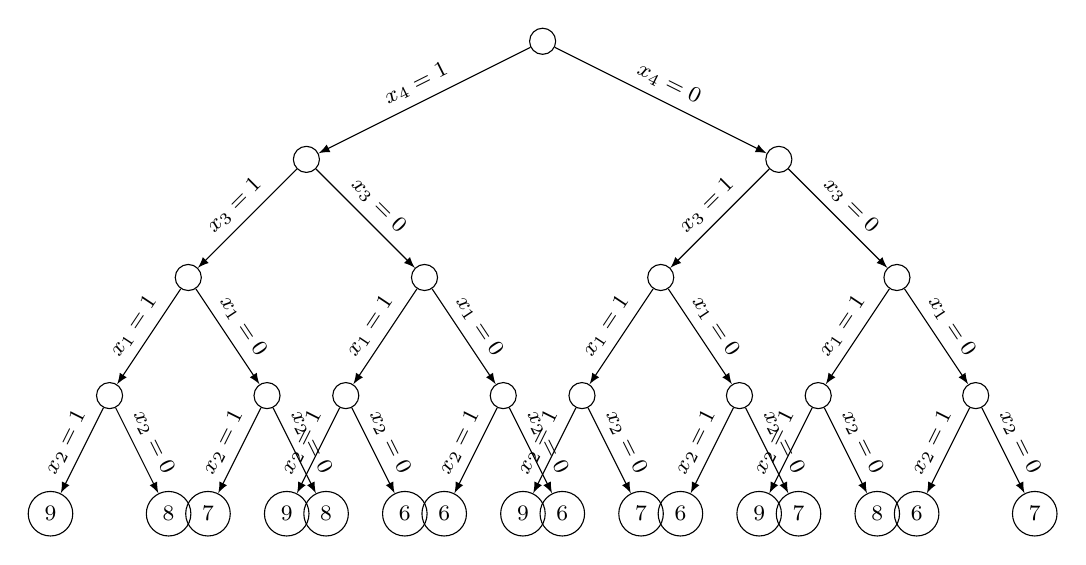
\begin{tikzpicture}[
    level/.style={sibling distance=60mm/#1}, 
    edge from parent/.style = {draw, -latex},
    every node/.style       = {font=\footnotesize},
    sloped,
    %rotate=90
]
\node [circle,draw] (root){}
  child {
  		node [circle,draw] (a) {} 		
    		child {
    			node [circle,draw] (b) {}
    			child {
    				node [circle,draw] (c) {}
    				child {
    					node [circle,draw] (d) {9}
    					edge from parent node [above] {\(x_2=1\)}
    				}
    				child {
    					node [circle,draw] (e) {8}
    					edge from parent node [above] {\(x_2=0\)}
    				}
    				edge from parent node [above] {\(x_1=1\)}
    			}
    			child {
    				node [circle,draw] (f) {}
    				child {
    					node [circle,draw] (g) {7}
    					edge from parent node [above] {\(x_2=1\)}
    				}
    				child {
    					node [circle,draw] (h) {8}
    					edge from parent node [above] {\(x_2=0\)}
    				}
    				edge from parent node [above] {\(x_1=0\)}
    			}
    			edge from parent node [above] {\(x_3=1\)}
    		}
    		child {
    			node [circle,draw] (i) {}
    			child {
    				node [circle,draw] (j) {}
    				child {
    					node [circle,draw] (k) {9}
    					edge from parent node [above] {\(x_2=1\)}
    				}
    				child {
    					node [circle,draw] (l) {6}
    					edge from parent node [above] {\(x_2=0\)}
    				}
    				edge from parent node [above] {\(x_1=1\)}
    			}
    			child {
    				node [circle,draw] (m) {}
    				child {
    					node [circle,draw] (n) {6}
    					edge from parent node [above] {\(x_2=1\)}
    				}
    				child {
    					node [circle,draw] (o) {6}
    					edge from parent node [above] {\(x_2=0\)}
    				}
    				edge from parent node [above] {\(x_1=0\)}
    			}
    			edge from parent node [above] {\(x_3=0\)}
    		}
    		edge from parent node [above] {\(x_4=1\)}
  }
  child {
  		node [circle,draw] (p) {}
  		child {
    			node [circle,draw] (q) {}
    			child {
    				node [circle,draw] (r) {}
    				child {
    					node [circle,draw] (s) {9}
    					edge from parent node [above] {\(x_2=1\)}
    				}
    				child {
    					node [circle,draw] (t) {7}
    					edge from parent node [above] {\(x_2=0\)}
    				}
    				edge from parent node [above] {\(x_1=1\)}
    			}
    			child {
    				node [circle,draw] (u) {}
    				child {
    					node [circle,draw] (v) {6}
    					edge from parent node [above] {\(x_2=1\)}
    				}
    				child {
    					node [circle,draw] (w) {7}
    					edge from parent node [above] {\(x_2=0\)}
    				}
    				edge from parent node [above] {\(x_1=0\)}
    			}
    			edge from parent node [above] {\(x_3=1\)}
    		}
    		child {
    			node [circle,draw] (x) {}
    			child {
    				node [circle,draw] (y) {}
    				child {
    					node [circle,draw] (z) {9}
    					edge from parent node [above] {\(x_2=1\)}
    				}
    				child {
    					node [circle,draw] (aa) {8}
    					edge from parent node [above] {\(x_2=0\)}
    				}
    				edge from parent node [above] {\(x_1=1\)}
    			}
    			child {
    				node [circle,draw] (ab) {}
    				child {
    					node [circle,draw] (ac) {6}
    					edge from parent node [above] {\(x_2=1\)}
    				}
    				child {
    					node [circle,draw] (ad) {7}
    					edge from parent node [above] {\(x_2=0\)}
    				}
    				edge from parent node [above] {\(x_1=0\)}
    			}
    			edge from parent node [above] {\(x_3=0\)}
    		}
  		edge from parent node [above] {\(x_4=0\)}	
  };
\end{tikzpicture}

	\item \includegraphics[width=\textwidth]{1b.pdf}

\end{enumerate}

\section*{Aufgabe 2}

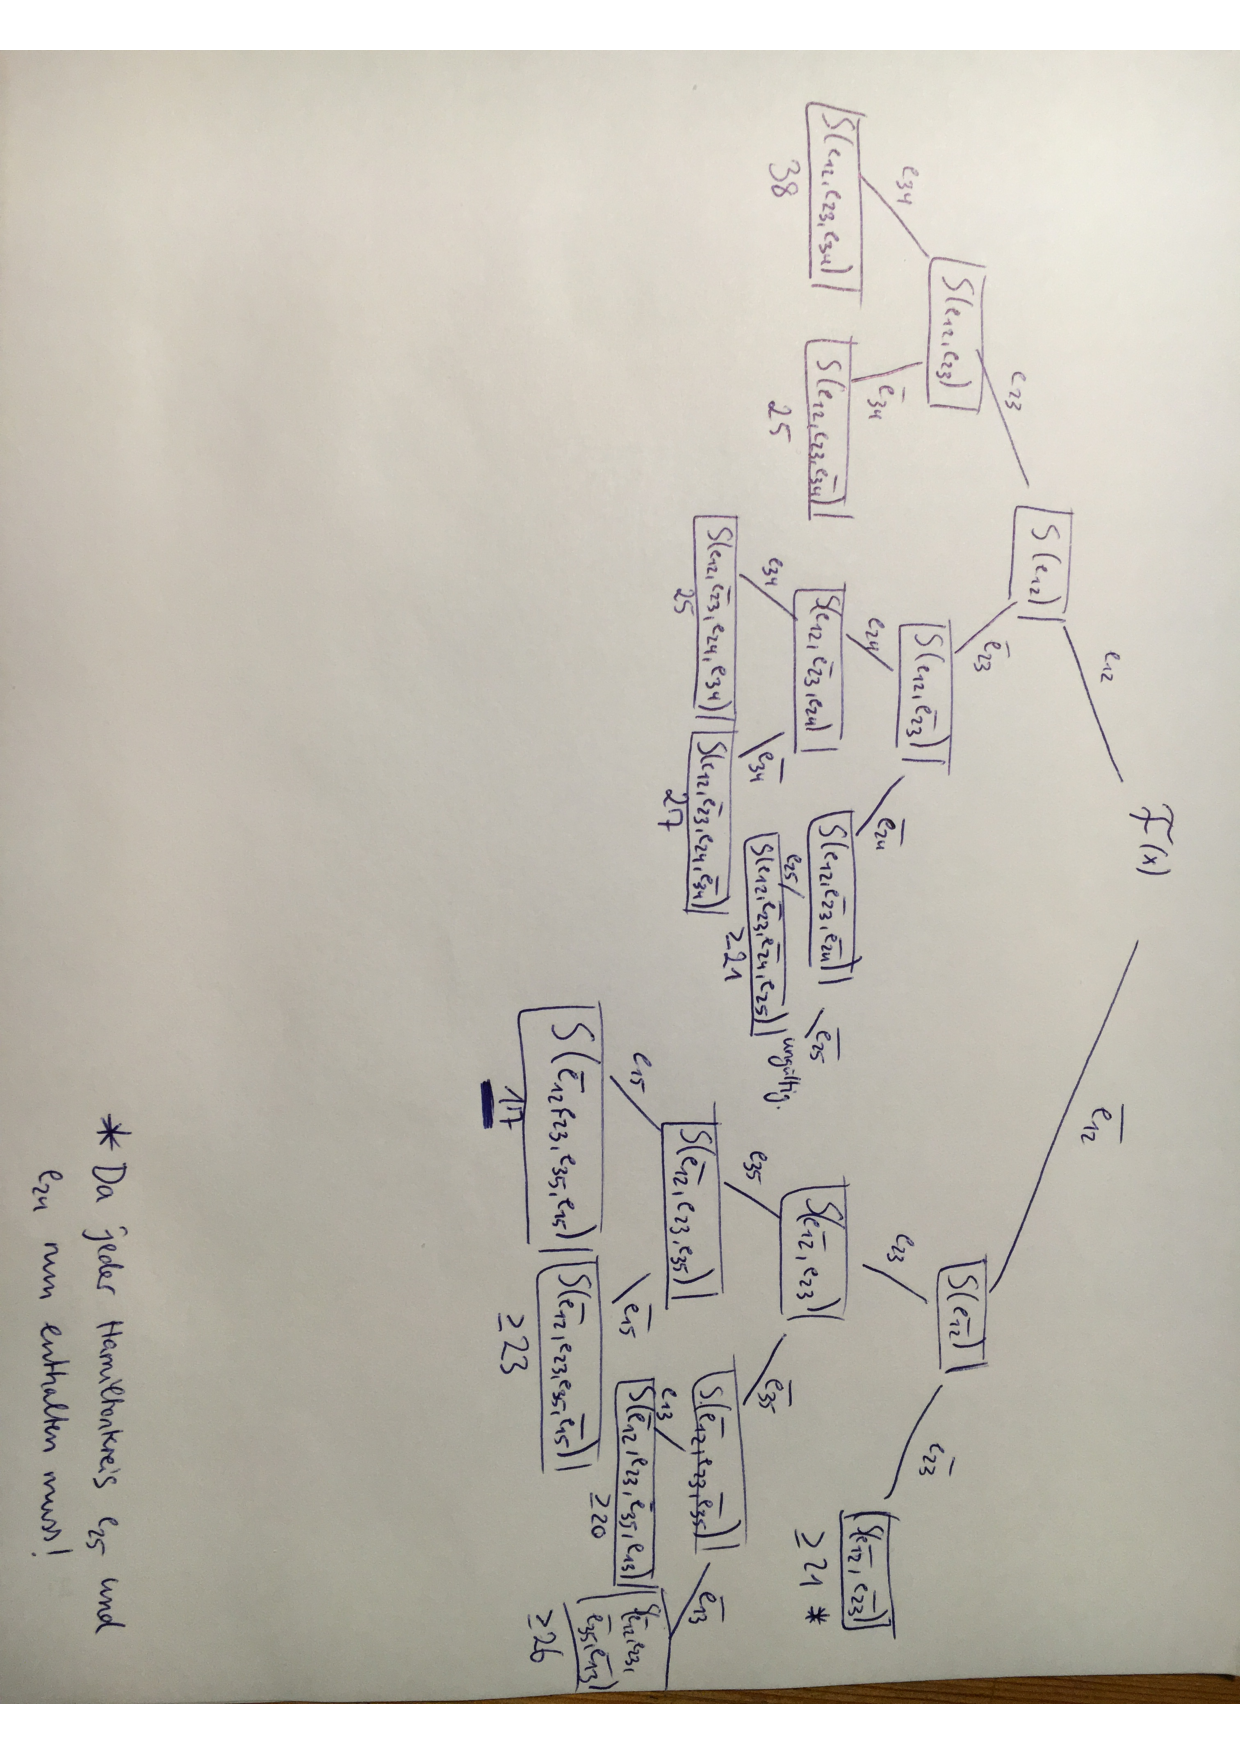
\includepdf{2.pdf}

\end{document}
